Wydajne zarządzanie zasobami jest kluczowym aspektem zapewnienia płynności działania gry. W tym podrozdziale omówimy strategie ładowania i zwalniania zasobów w zależności od potrzeb sceny. Przyjrzymy się tematom takim asynchroniczne ładowanie czy korzyści płynące z użycia wzorca \textit{puli obiektów}.

\subsubsection{Asynchroniczne Ładowanie}
Asynchroniczne ładowanie sceny jest kluczowym elementem optymalizacji gier, umożliwiając płynne przejścia między różnymi fragmentami rozgrywki. W tym kontekście przedstawiamy skrypt \texttt{SceneLoader.cs}, który implementuje asynchroniczne ładowanie sceny w grze.
\begin{codebox}
\begin{lstlisting}[language={[Sharp]C}, label={listing:SceneLoader.cs}]
public class SceneLoader : MonoBehaviour
{
    // ... (Remaining part of the script)

    public IEnumerator LoadScene_Coroutine(int index)
    {
        AsyncOperation asyncOperation = SceneManager.LoadSceneAsync(index);
        asyncOperation.allowSceneActivation = false;
        float progress = 0;
        
        while (!asyncOperation.isDone)
        {
            progress = Mathf.MoveTowards(progress, asyncOperation.progress, Time.deltaTime);
            progressSlider.value = progress;
            
            if (progress >= 0.9f)
            {
                progressSlider.value = 1;
                asyncOperation.allowSceneActivation = true;
            }
            
            yield return null;
        }
    }
}
\end{lstlisting}
\end{codebox}
\captionof{lstlisting}{Klasa SceneLoader obsługująca asynchroniczne przechodzenie między scenami}
Skrypt ten umożliwia dynamiczne ładowanie sceny, co jest szczególnie użyteczne przy dużych i rozbudowanych projektach. Kluczowym elementem jest użycie klasy \texttt{AsyncOperation}, która pozwala na asynchroniczne ładowanie sceny w tle, bez blokowania głównego wątku gry.
\textbf{Elementy kluczowe skryptu:}
\begin{itemize}
\item \textbf{LoaderUI:} Obiekt reprezentujący interfejs użytkownika (UI) wykorzystywany podczas ładowania sceny.
\item \textbf{progressSlider:} Pasek postępu ładowania sceny, umożliwiający informowanie gracza o aktualnym stanie procesu.
\item \textbf{gOToDeactivate:} Obiekt do dezaktywacji podczas ładowania sceny, co może być przydatne, aby ukryć niepotrzebne elementy w trakcie przejścia między scenami.
\item \textbf{LoadScene:} Metoda rozpoczynająca proces ładowania sceny. Wywołuje \texttt{LoadScene\_Coroutine} w ramach coroutine.
\item \textbf{LoadScene\_Coroutine:} Coroutine odpowiedzialna za asynchroniczne ładowanie sceny. W trakcie procesu aktualizuje pasek postępu, a po osiągnięciu 90\% pozwala na aktywację sceny.
\end{itemize}
Użycie asynchronicznego ładowania sceny poprzez ten skrypt pozwala na zachowanie płynności rozgrywki nawet w przypadku dużych i złożonych scen, jednocześnie umożliwiając informowanie gracza o postępie za pomocą paska ładowania. Skrypt osiąga stan 90\% ładowania, a następnie pozwala na aktywację sceny. Ograniczenie ładowania do 90\% zanim scena zostanie aktywowana ma na celu zminimalizowanie zakłóceń związanych z ostatecznym przejściem do nowej sceny, umożliwiając jednocześnie aktualizację interfejsu użytkownika i przygotowanie do gry. Jest to istotny element optymalizacji, który przyczynia się do lepszych doświadczeń graczy.

\subsubsection{Object Pooling}
\textit{Object Pooling} umożliwia efektywne ponowne wykorzystanie obiektów w grze, zamiast dynamicznego tworzenia i niszczenia ich. Podejście to pomaga zminimalizować obciążenie systemu, zwłaszcza w przypadku obiektów, które są często tworzone i usuwane, takich jak efekty cząsteczkowe, wskaźniki obrażeń, popupy z obrażeniami czy rany po pociskach. \\ \\
Skrypt \texttt{ObjectPoolManager.cs} jest centralnym elementem zarządzającym pulą obiektów. Jeżeli interesuje Cię sama implementacja funkcji do tworzenia puli obiektów oraz tej odpowiedzialnej za ich powrót do puli to sugerujemy powrót do podsekcji \nameref{subsubsec:objPoolPattern} gdzie możesz znaleźć code snippet, którego szukasz! Poniżej przedstawiono główne funkcje skryptu:
\begin{itemize}
    \item \textbf{SpawnObject:} Funkcja ta służy do tworzenia obiektów z puli. Sprawdza, czy dany obiekt już istnieje w puli. Jeśli nie, tworzy nowy obiekt; jeśli tak, ponownie go aktywuje i umieszcza na odpowiedniej pozycji.
    \item \textbf{ReturnObjectToPool:} Funkcja odpowiada za zwrot obiektu do puli po zakończeniu jego używania. Obiekt jest dezaktywowany i dodawany z powrotem do puli.
    \item \textbf{SetParentObject:} Funkcja ta ustawia rodzica dla danego obiektu w zależności od jego typu. Pomaga to w utrzymaniu porządku w hierarchii obiektów w scenie.
\end{itemize}
Dodatkowo, skrypty które znajdziesz poniżej prezentują konkretne przypadki użycia \textit{puli obiektów} w akcji: \label{subsubsec:objPoolExamples}
\begin{itemize}
    \item Skrypt \textbf{ReturnParticlesToPool.cs:} Skrypt ten reprezentuje konkretny przypadek użycia \textit{puli obiektów} w kontekście efektów cząsteczkowych. Po zakończeniu emisji cząsteczek wywołuje funkcję zwracającą obiekt do puli.
    \begin{codebox}
    \begin{lstlisting}[language={[Sharp]C}, label={listing:ReturnParticlesToPool.cs}]
    public class ReturnParticlesToPool : MonoBehaviour
    {
        private void OnParticleSystemStopped()
        {
            ObjectPoolManager.ReturnObjectToPool(gameObject);
        }
    }
    \end{lstlisting}
    \end{codebox}
    \captionof{lstlisting}{Zwrócenie obiektu do puli po zakończeniu trwania efektu systemu cząsteczkowego}
\end{itemize}
\begin{itemize}
    \item Skrypt \textbf{ReturnToPoolAfterTimer.cs} Ten skrypt ilustruje użycie \textit{puli obiektów} w kontekście czasowego zwalniania zasobów. Po aktywowaniu obiektu, rozpoczyna odliczanie czasu i po upływie określonego czasu, zwraca obiekt do puli.
    \begin{codebox}
    \begin{lstlisting}[language={[Sharp]C}, label={listing:ReturnToPoolAfterTimer.cs}]
    public class ReturnToPoolAfterTimer : MonoBehaviour
    {
        public float timeToDespawn = 1f;
        private Coroutine _timerCoroutine;

        private void OnEnable()
        {
            _timerCoroutine = StartCoroutine(ReturnToPoolAfterTime());
        }
        private IEnumerator ReturnToPoolAfterTime()
        {
            float elapsedTime = 0f;

            while(elapsedTime < timeToDespawn)
            {
                elapsedTime += Time.deltaTime;
                yield return null;
            }

            ObjectPoolManager.ReturnObjectToPool(gameObject);
        }
    }
    \end{lstlisting}
    \end{codebox}
    \captionof{lstlisting}{Zwrócenie obiektu do puli po upływie określonego czasu}
\end{itemize}
\begin{itemize}
    \item Skrypt \textbf{ReturnToPoolOnAnimationEnd.cs:} Skrypt ten prezentuje wykorzystanie \textit{puli obiektów} w kontekście zwalniania zasobów po zakończeniu animacji. Po zakończeniu animacji obiektu, rodzic tego obiektu zostaje zwrócony do puli.
    \begin{codebox}
    \begin{lstlisting}[language={[Sharp]C}, label={listing:ReturnToPoolOnAnimationEnd.cs}]
    public class ReturnToPoolOnAnimationEnd : MonoBehaviour
    {
        public void DestroyParent()
        {
            GameObject parentObject = gameObject.transform.parent.gameObject;
            ObjectPoolManager.ReturnObjectToPool(parentObject);
        }
    }
    \end{lstlisting}
    \end{codebox}
    \captionof{lstlisting}{Klasa ReturnToPoolOnAnimationEnd wykorzystywana do zwrócenia obiektu do puli po zakończeniu trwania animacji przy użyciu zdarzeń animacji Unity}
\end{itemize}
Poniżej znajdziesz konfiguracje obiektów w zależności od sposobu w jaki możesz je dodać do systemu \textit{puli obiektów} oraz przykład podmiany wbudowanych i kosztownych funkcji silnika Unity, czyli \textit{Instantiate} oraz \textit{Destroy}.
\begin{figure}[h]
    \centering
    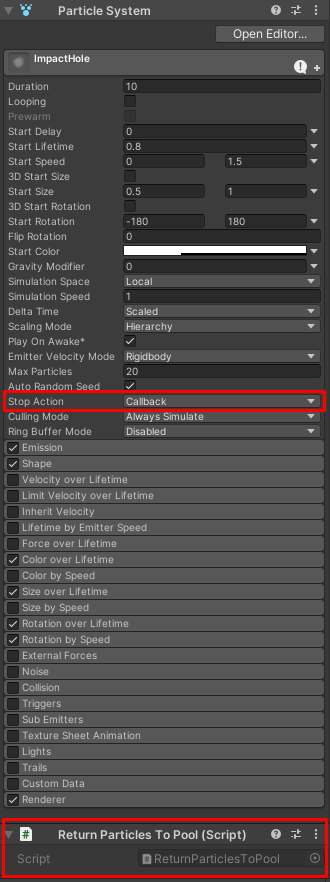
\includegraphics[scale=0.55]{Images/particlesObjPoolSetup.png}
    \caption{Konfiguracja obiektu Particle System, który powinien wrócić do puli obiektów po zakończeniu emisji cząsteczek}
\end{figure}
\FloatBarrier
\begin{figure}[h]
    \centering
    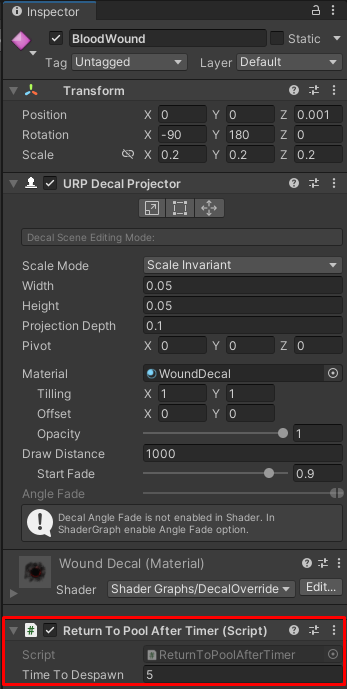
\includegraphics[width=0.5\linewidth]{Images/timerObjPoolSetup.png}
    \caption{Konfiguracja obiektu, który ma wrócić do puli obiektów po upływie czasu}
\end{figure}
\FloatBarrier
\begin{figure}[h]
    \centering
    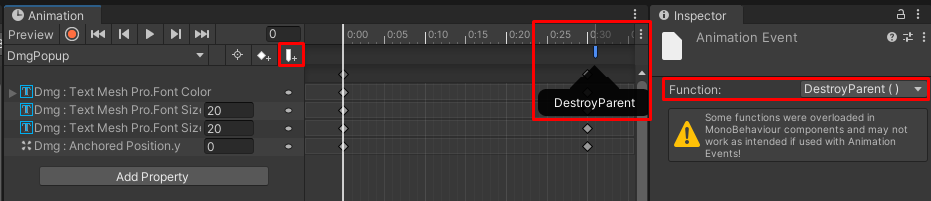
\includegraphics[width=1\linewidth]{Images/animObjPoolSetup.png}
    \caption{Konfiguracja obiektu, który ma wrócić do puli obiektów po zakończeniu odtwarzania animacji}
\end{figure}
\FloatBarrier
\begin{figure}[h]
    \begin{codebox}
    \begin{lstlisting}[language={[Sharp]C}, label={listing:DISystem.cs}]
    public class DISystem : MonoBehaviour
    {
        [SerializeField] private GameObject indicatorPrefab;
        [SerializeField] private RectTransform holder;

        // ... (Remaining part of the script)
        
        private void Create(Transform target)
        {
            // ... (Remaining part of the function)

            GameObject indicator = ObjectPoolManager.SpawnObject(indicatorPrefab, Vector3.zero, Quaternion.identity, holder);
            
            // ... (Remaining part of the function)
        }
    }
    \end{lstlisting}
    \end{codebox}
    \captionof{lstlisting}{Przykład podmiany funkcji Instantiate w skrypcie DISystem.cs na nowo utworzoną i zoptymalizowaną SpawnObject z klasy ObjectPoolManager}
\end{figure}
\begin{figure}[h]
    \begin{codebox}
    \begin{lstlisting}[language={[Sharp]C}, label={listing:DamageIndicator.cs}]
    public class DamageIndicator : MonoBehaviour
    {
        // ... (Remaining part of the script)
        
        private IEnumerator Countdown()
        {
            // ... (Remaining part of the function)

            unRegister();
            ObjectPoolManager.ReturnObjectToPool(gameObject);
        }
    }
    \end{lstlisting}
    \end{codebox}
    \captionof{lstlisting}{Przykład podmiany funkcji Destroy w skrypcie DamageIndicator.cs na nowo utworzoną i zoptymalizowaną ReturnObjectToPool z klasy ObjectPoolManager}
\end{figure}